\documentclass[smallextended]{svjour3}       % onecolumn (second format)
\smartqed  % flush right qed marks, e.g. at end of proof
\usepackage{easy-todo}
\usepackage{mathptmx}      % use Times fonts if available on your TeX system
\usepackage{times}
\usepackage[utf8]{inputenc}
\usepackage{url}
\usepackage{latexsym}
\special{papersize=210mm,297mm} % to avoid having to use "-t a4" with dvips 
%\setlength\titlebox{6.5cm}  % You can expand the title box if you really have to
\usepackage{graphicx}
\usepackage{placeins}
\usepackage{framed}
\usepackage{pbox}
\usepackage{amsmath}
\usepackage{supertabular}
\usepackage{algorithm} 
\usepackage{algpseudocode} 
\usepackage{caption}
\usepackage{gb4e}
\usepackage{natbib}


\let\proof\relax
\let\endproof\relax
\usepackage{amsthm}
\newtheoremstyle{break}
  {\topsep}{\topsep}%
  {\itshape}{}%
  {\bfseries}{}%
  {\newline}{}%
\theoremstyle{break}
\newtheorem{exmp}{Example}[section]

\DeclareMathOperator*{\argmin}{arg\,min}
\DeclareMathOperator*{\argmax}{arg\,max}

\title{Language-independent classifier-based modelling of source-side context information in Statistical Machine Translation}
\titlerunning{Source-side context in SMT}


\author{Maarten van Gompel \& Antal van den Bosch \\
 Centre for Language Studies \\
  dboud University Nijmegen \\
  {\tt proycon@anaproy.nl}}

%\date{}


\begin{document}
\maketitle

\begin{abstract} 
  We present in-depth research into the modelling of source-side
  context to improve Phrase-based Statistical Machine
  Translation. Statistical Machine Translation systems typically
  consist of a translation model and a language model. The former maps
  phrases in the source language to the target language, without
  regard for the context in which the source phrases occur. The latter
  models just the target language, and acts as a target-side model of
  context information after translation. We attempt to independently
  reproduce a line of existing research and test whether considering
  context information directly in the translation model has a positive
  effect on translation quality.  We furthermore investigate various
  ways classifier-based models can be integrated into Statical Machine
  Translation.  We will use proven techniques from Word Sense
  Disambiguation, effectively integrating WSD techniques in
  Statistical Machine Translation. Our approach is
  language-independent: we do not employ any explicit linguistic
  features computed by part-of-speech taggers, word sense
  disambiguation systems, supertaggers, or parsers, as used by
  previous work.
\end{abstract}

\section{Introduction}

In Phrase-based Statistical Machine Translation (SMT) the problem of
translating an input sentence from a source language to a target language is
perceived as a game of probabilities and a search for the most probable
translation option.  These probabilities are expressed in a number of models
that specialize in a certain aspect relevant to the translation process. The
``phrase-based'' characteristic is due to phrases being the building blocks of
the translation model. This can be contrasted to earlier approaches in
Statistical Machine Translation which started as word-based.  Phrases in this
sense have to be perceived simply one or more words, i.e.  n-grams of variable
length (including unigrams). Moreover, they are not at all required to form a
proper linguistic constituent of any kind.

Two models are at the core of phrase-based SMT: first there is the translation
model which maps the translation phrases in the source language ($s$) to
phrases in target language ($t$), this mapping is expressed as a vector of
probabilities, most notably $P({phrase}_s|{phrase}_t)$ and
$P({phrase}_t|{phrase}_s)$. This component can be seen to model the notion of
``semantic faithfulness''; if you translate a phrase from one language to
another, you want the meaning to be preserved as accurately as possible. The
second core model is the language model, this model in monolingual in nature
and models \emph{the target language}. It models what words are likely to
follow others and can be interpreted as modelling the ``syntactic fluency''
notion of translation; a translation should be in a natural word-order and
sound natural. A Machine Translation \emph{decoder} optimises a log-linear
model of these two, and additional other, models. Given an input sentence in
the source language, it searches through a vast space of all ``possible''
translation options, most non-sensical, for a path maximising the probabilities
according to each of the models, taking into account different weights they may
be assigned.

The study we currently present focusses on the role of surface-form context
information in this SMT process. The Language Model effectively models context
for the target language, it makes sure that a translated phrase fits nicely
along other translated phrases. But in SMT there is no component modelling
context for the source-language, whereas intuitively source-side context may
provide a powerful cue for translation. Consider the word ``bank'' and its
Spanish translation in examples~\ref{ex:bank1} and \ref{ex:bank2}.

\begin{exe} %gb4e package
\ex \textbf{English:} I don't trust the bank. \\
    \textbf{Spanish:} No me fio del banco.
\label{ex:bank1}

\ex \textbf{English:} The boat headed towards the bank of the river. \\
    \textbf{Spanish:} El barco se dirigió hacia la orilla del río.
\label{ex:bank2}
\end{exe}

The same English word, ``bank'' may express multiple semantic senses, some of
which are expressed by different words in Spanish. Source-side context
information may provide valuable clues to what sense is being employed, and
therefore what translation is correct.  The words ``boat'' and the phrase ``of
the river'' in example \ref{ex:bank2} make it pretty clear that we are using
bank in its maritime sense. Example \ref{ex:bank1} is less obvious, but the
word ``trust'' could be seen to be a cue when the noun ``bank'' denotes a
financial institution.

These examples are meant to illustrate the intuition that is behind our
research hypothesis. We hypothesise that the inclusion of source-side context
information in the translation model improves translation results, as the
context helps in providing a more accurate disambiguation. A counter-hypothesis
to this would be that whilst source-side context information is not modelled
explicitly, it is implicitly captured by the combination of translation model
and language model, and explicit modelling has no added value.

There is clear and obvious overlap between what we do here and the field of
Word Sense Disambiguation (WSD). We effectively test an integration of proven
techniques from WSD in Statistical Machine Translation, and apply these to
phrases rather than just words.

WSD systems often employ a variety of linguistic features. The focus of our
study, however, is to be independent of the explicit computation of
linguistically abstract features with language-dependent tools such as
part-of-speech taggers, supertaggers, or dependency parsers
\cite{Rejwanul+11}. 
%We are interested only in the surface
%forms, the text as-is, and stay as close as possible to vanilla Phrase-Based
%Statistical Machine Translation, without using any language-specific external
%resources. 
In this fashion, we attempt to assess the merit of source-side
context information as purely as possible.

Not introducing extra data for the translation system means our goals have to
be set more modest as well. We may not expect the same gains as are achieved by
introducing extra data from linguistic preprocessors.

\section{Previous research}

The idea to integrate WSD approaches in SMT is not new, nor is the idea to use
source-side context information to disambiguate in translation. Various studies
have been conducted with mixed results. In the early days of SMT,
\cite{GarciaVarea+02} already explicitly modelled source-side context in a
maximum entropy model for word-based SMT, and report slightly improved error
rates on a translation task.

\cite{CarpuatWu05} were the first to directly tackle the question whether
full-scale WSD models were beneficial to translation quality when integrated in
SMT systems, and thus their work forms important foundation for our own study.
Their approach uses an ensemble classification model that integrates
position-sensitive, syntactic, and local collocational features, which has
proven itself in competitive WSD tasks. This includes linguistic features such
as part-of-speech tags and lemmas, as well as more complex syntactic relations.
They test for a single Chinese-to-English test-set only, and only use BLEU,
which raises some questions on whether their conclusions would hold on
different language pairs, test sets, and using different evaluation metrics.

\cite{CarpuatWu05} place strong focus on the WSD model rather than the SMT
model, whereas we place more focus on the SMT model and the integration method,
and keep the ``WSD-model'' relatively simple. Furthermore, the method they
employ a simpler word-based form of Statistical Machine Translation and the
level of integration seems limited.

Despite their efforts, they reach the surprising conclusion that inclusion of
WSD techniques does \emph{not} yield better translation quality. Will these
results hold in a more modern Phrase-based Statistical Machine Translation
approach?

Two years later they expanded their study to full phrasal units
\citep{CarpuatWu07} and, for the first time, found results that did support the
hypothesis that SMT benefits from the integration of WSD techniques. They now
focus on better integration in \emph{phrase-based} SMT: ``Rather than using a
generic SenseEval model as we did in \cite{CarpuatWu05}, here both the WSD
training and the WSD predictions are integrated into the phrase-based SMT
framework.'' \citep{CarpuatWu07}. They also broaden their use of evaluation
metrics, yet still test on only Chinese to English.

The work of \cite{Gimenez+07} is similar, they use support vector machines to
predict the phrase translation probabilities for the phrase-translation table
component of SMT, rather than relying on the context-unaware Maximum Likehood
Estimate the statistical process produces. The feature vector for their
classifiers consists of both local context as well as global context features.
In addition to the surface forms of the words, they do rely on shallow
linguistic features such as Part-of-Speech tags and lemmas. They conduct a
manual evaluation judged on fluency and adequacy, and conclude that considering
context improves adequacy, yet does not benefit fluency. They remark that the
integration of the classifier probabilities in an SMT framework needs further
study, which is something that will indeed be a focus in our present study.

The year 2007 saw a culmination of various studies integrating WSD techniques in
SMT using classifiers. A third study in this trend was \cite{Stroppa+07}. They
have a strong focus on the word form, as does this present study, and add only
part-of-speech features. On IWSLT 2006 data for Chinese-English and
Italian-English, they achieve a significant improvement for the former, whereas
the BLEU score for the latter fails to pass the significance test. We will
attempt to reproduce these experiments in this study.

Source-context aware translation has also been attempted outside of the
predominant statistical machine translation framework. \cite{MBMT} implement a
simple form of example-based machine translation that is word-based and relies
chiefly on classifiers for the translation model component. Two studies derive
from the same concept while transcending a word-based paradigm:
\cite{MARKERBASED} use chunks delimited by common markers, and \cite{PBMBMT}
attempts a full extension to phrases similar to SMT. Although positive results
are achieved in the latter study, it does not rival state-of-the-art SMT.

The most important and complete study we build upon is \cite{Rejwanul+11},
which in turn draws from the majority of the aforementioned studies, and
provides an extensive comparison between them. Their study finds that including
such linguistically-informed contextual features in general produces
improvements.  The main contrast between our study and theirs is that they
focus on a variety of linguistically-informed contextual features, whereas we
depart from a language-independent angle and intend to settle some of the
conflicting reports whether this may lead to an improvement in translation
quality. A notable focus in our study will be possible methods of integrating the
classifier probabilities in the SMT, as recommended also by \cite{Gimenez+07}.


\section{Methodology}
\label{ref:methodology}

Like most of the latest studies before us, we approach the machine translation
problem in a phrase-based fashion, which has superseded the simpler word-based
based paradigm for quite some time. This means that phrases, defined as a
sequence of one or more words (that need not form a linguistic entity in any
way!), form the basic building blocks of our translation model. The problem of
translating a sentence is decomposed into the problem of translating its phrasal
subparts and combining the results in the best order.

In describing our methodology, we first focus on the problem of phrasal
translation, adding in the source-side context component. This shall be done
using classifiers. Then we address how this can be integrated into a
phrase-based Stastiscal Machine Translation decoder, which also takes care of
ordering aspect. 


\subsection{Modelling source-side context with classifiers}

In line with several previous studies \citep{Rejwanul+11,PBMBMT,
Stroppa+07,MARKERBASED}, we make use of memory-based classifiers to build a
translation model informed by source-side context information. More
specifically, we will be using IB1 \citep{IB1}, an implementation of k-Nearest
Neighbours; IGTree \citep{IGTree}, an optimised and lossless tree-based approximation thereof;
and TRIBL2, a mixture model of the two. 

These algorithms are all implemented in the
software Timbl \citep{TIMBL}\footnote{\url{http://ilk.uvt.nl/timbl}} and
are well-suited for symbolic data and highly multivariate classes.
Moreover, memory-based classification has been a proven solution in the field
of Word Sense Disambiguation \citep{SENSEVAL2,WSD2}.

When speaking of the $k$ nearest neighbours in the implementation of IB1,
IGTree and TRIBL2, we are actually referring to the neighbours at nearest
distance $k$. So even with $k=1$ we may be talking about multiple data points
that are all at equal distance.

%(these two paragraphs are paraphrased from my PBMBMT thesis, not sure to cite
%or prevent for risk of over-self-citation here)
IGTree compresses the instance base into an ordered decision tree structure at
training time, and issues look-ups in this tree structure at test time. Unlike
other top-down induced decision tree methods such as C4.5, features in IGTree
are tested in a fixed order. This is computed \emph{only once and in advance}
for all features. This order is determined using metrics such as
\emph{information gain} or \emph{gain ratio}. They determine the relative
informativeness or disambiguating power of the feature and provide a ranking of
all features. 

IGTree's performance relies on the differences in information gain between
features. If these are small then IGTree may perform significantly below IB1
\citep{TIMBL}. A hybrid approach called TRIBL2 \citep{TIMBL} starts out with
IGTree and switches to a IB1 variant when a value mismatch occurs in the tree.
In this study, we therefore opt to use TRIBL2 over plain IGTree, but only when
using IB1 would have a prohibitively large impact on performance.

In our classifier-based translation model we will be modelling the probability
of a target phrase ($t$) given a source phrase ($s$) and context information
($C$). We can thus express this as $P(t|s,C)$.  \cite{Stroppa+07} state that
direct estimation of this probability using relative frequencies would result
in overestimation of large phrases, and that therefore a smoothing factor is
required. They proceed to say that through memory-based classification we
implicitly introduce precisely such a smoothing factor.

Given a source phrase and context information, the classifier yields classes
corresponding to target phrases, with an associated weight. After
normalization, these can be considered a posterior distribution of
target phrases. 

We primarily focus on the modelling of local context, i.e. words in the
immediate vicitinity of the source phrase. Take $w_0$ to be the first word of
the source phrase $s$, then for a local context size of $n$ words to the left and
$m$ to the right we construct the feature vector $C$ as follows:

\begin{equation}
  C = \langle w_{-n} .. w_{-1} , s , w_{|s|+1} .. w_{|s|+m} \rangle
\end{equation}

For context words out of the sentence's bounds, placeholders are used instead.

Now there are two ways in which we can construct a classifier:

\begin{itemize}
  \item \textbf{Monolithic classifier} -- One aggregated classifier for all
    source phrases.
  \item \textbf{Classifier experts} -- One classifier per source phrase.
\end{itemize}

In this study we will use and compare both methods, which is, for the task at
hand, the first such a comparison in the literature as far as we know.

For the monolithic classifier, the first feature in the ranking will always be
$s$. Nevertheless, it is quite conceivable that a match for the context is not
found and the classifier proceeds to match on another feature. To prevent
situations in where the classifier falls back to a completely different source
phrase, and thus comes up with unrelated translation options, we enforce that
the source phrases need to match exactly, which is what \cite{Stroppa+07} do as
well.

For the classifier experts, on the other hand, the source phrase is the least
powerful feature in the ranking, as it is shared amongst all instances. We
therefore simply omit it from the feature vector.

\subsection{Training}

The translation model is trained on parallel corpus data. We follow a common
MT pipeline and at the end derive classifier training data.

Given a tokenised and sentence-aligned parallel corpus, we iteratively learn
word alignments using GIZA++ \citep{GIZA}. Then we identify and extract phrase
pairs using the {\em grow-diag-final}\/ algorithm \citep{OchNey2003}. The
result is a phrase-translation table mapping source phrases to target
phrases, along with associates scores which we will discuss in the next
section. This phrase-translation table effectively constitutes the translation
model.

The translation model would be finished if we would want to leave it to be
non-context-informed. We have some additional steps to perform to train our
context-informed classifiers. We take the phrase-translation table, along with
the parallel corpus, as a basis for extracting training instances.

We build indexed pattern models of all source phrases and target phrases that
occur on their respective side the parallel corpus, and which also occur in the 
phrase-translation table. An indexed pattern model maps each distinct phrase to
the locations in the corpus where it occurs.  Additionally, a reverse index is
included in the model for the target-side of the corpus, which maps any given
$(sentence, token)$ position to a set phrases that begins at that position.
This is computed using the software \emph{colibri-core}
\footnote{http://proycon.github.io/colibri-core}, which takes care of a
losslessly compressed in-memory representation for all phrases, and allows us
to cope with large corpora.

Given these two pattern models $M_{source}$ and $M_{target}$ we can quickly and
efficiently extract the context for each phrase pair, as shown in simplified
form in Algorithm~\ref{alg:featureextract}.  

\begin{algorithm}
\caption{Algorithm for feature extraction for training classifiers.  Take $n$
again to be the left context, $m$ to be the size of the right context, and
$w{(i,j)}$ to denote the word in the source corpus in sentence $i$, token $j$.
The vector $C$ represents the context information and constitutes the feature
vector.  The algorithm will return a list containing two-tuples $(C,t)$.  }
\label{alg:featureextract}
\begin{algorithmic}
\State instances $\gets []$
\For {$(s \in M_{\text{source}}, t \in M_{\text{target}})$}
  \For {$i \in (M_{\text{source}}[s] \cap M_{\text{target}}[t])$}
    \For{$j \in M_{\text{source}}[s][i]$}
        \State $C \gets \langle w_{i,j-n} \ldots w_{i,j-1}, s, w_{i,j+|s|+1} \ldots w_{i,j+|s|+m} \rangle$
        \State \Call{instances.append}{$(C, t)$} 
      \EndFor
  \EndFor
\EndFor \\
\Return{instances}
\end{algorithmic}
\end{algorithm}
    
This algorithm is implemented in \emph{colibri-mt}
\footnote{https://github.com/proycon/colibri-mt}.

The return instances can be stored directly, either in a single model for the
monolithic approach or in separate models for each $s$ for the classifier
expert approach. A final training phase then computes the feature ranking and
transforms this data into the instance base format required for Timbl.

When extra training data for the classifier(s), it may well happen that either
1) an $(s,t)$ pair only occurs once, or 2) a pattern $s$ occurs in multiple
context but all map to the same $t$. In such cases, a context-informed
classifier clearly has no added value and therefore such instances are omitted from the training data.  

\subsection{Integration in an SMT Decoder}
\label{sec:smtintegration}

The task of an SMT decoder is to find the best translation amongst a vast pool
of possible translation hypotheses. The best translation hypothesis is the
translation hypothesis that maximises a log linear combination and is sought
after in a beam-search algorithm. This log-linear combination draws from
various models, such as a translation model (i.e. the phrase-translation
table), a target-language model, and optionally additional models such as a
distortion model or word-reordering model. 

The SMT model is generally expressed as in equation~\ref{eq:smtmodel}, take $e$
to be the translation in the target language, and $f$ to be the sentence to be
translated, in the source language.

\begin{equation}
\argmax_e p(e|f) = \argmax_e p(e|f)p(e)
\label{eq:smtmodel}
\end{equation}

Bayes' rule inverts the problem into two factors, the former corresponding to
the translation model, and the latter corresponding to the language model. 

The translation model is a mapping of the set of source phrases ($S$) to the
set of target phrases ($T$). Each phrase-pair $(s,t)$ where $s \in S$ and $t
\in T$ is in described by a score vector indicating the likelihood of
translation. This score vector most notably consists of the probabilities
$p(s|t)$ and $p(t|s)$. In addition, lexical weighting probabilities $lex(s|t)$
and $lex(t|s)$ express the probability of a phrase-pair word-by-word, and are
often included as components in the score vector. During decoding, the total
score of the translation model and other models is expressed as a log-linear
combination, in which different weights can be assigned to each of the
components of the score vector. These weights are meta-parameters to the task and
are typically optimised automatically on development data using for instance
Minimum Error Rate Reduction \citep{MERT}.

The probability $p(t|s)$ is the one we are interested in. Recall that the
classifiers seek to model $p(t|s,C)$, where $C$ constitutes the vector of
context information. The hypothesis under investigation in the present study is
that $p(t|s,C)$ is a more accurate measure than $p(t|s)$.

The state-of-the art SMT decoder used in the majority of MT studies is Moses
\citep{MOSES}. However, it offers no facilities to take source-side context
information in account. We had to consider three options to achieve our goal of
integrating source-side context : 1) creating a new decoder; 2) enhancing
Moses; or 3) using a bypass method. Although we initially set out to create a
new decoder, it proved to be too difficult to attain the same quality as Moses.
We therefore decided, in line also with most of the literature, to follow the
third option, it is easiest and allows us to use Moses as a black box.

The bypass method is our \emph{discriminative translation filtering}
step \citep{Rejwanul+11}, it performs context-aware classification in a
pre-processing step, namely through alteration of the phrase-translation table,
and bypasses the need to alter the decoder in any way. We effectively take each
sentence individually and ensure that the entries in the phrase-translation
table are explicitly tuned to the source-side context. The output of the
classifier(s) acts as the filter and constrains the translations options, as
well as adjusts the score vector. Each instance of a source phrase will get a
separate entry in the phrase-translation table, as opposed to one source phrase
applying to all instances in the test data. 

To achieve this, each source phrase in the phrase-translation table is replaced
by a representation of its position in the test data, e.g.  $(1,0)$ for first
sentence, first word.  This is done using the software \texttt{colibri-mt}. It
creates an indexed pattern model on the test data, constrained by the phrases
in the phrase-translation table. This thus constitutes a mapping of all distinct
source phrases in the phrase-translation table to the indices in the test
corpus that are instances of these phrases.

Subsequently we invoke the classifier(s) and construct the altered
phrase-translation table as shown in Algorithm~\ref{alg:contextmoses}.

\begin{algorithm}
\begin{algorithmic}
  \For {$s \in M_{\text{test}}$}
  \For {$(i,j) \in M_{\text{test}}[s]$}
    \State $C \gets \langle w_{i,j-n} \ldots w_{i,j-1}, s, w_{i,j+|s|+1} \ldots w_{i,j+|s|+m} \rangle$
    \State $[(t, p(t|s,C) )] \gets$ \Call{classify}{$s,i,j,C$}
    \State {\Call {appendtophrasetable}{$s,i,j,[(t, p(t|s,C)]$}}
  \EndFor
\EndFor
\end{algorithmic}
\caption{Classifier invocation on test data. Take $M{\text{test}}$ to be the pattern
model of the test data, i.e. a map of source phrases occuring in the test
data, and $[(t,p(t|s,C))]$ to be a list of translation options ($t$) with
associated probability $p(t|s,C)$.}
\label{alg:contextmoses}
\end{algorithm}

In Algorithm~\ref{alg:contextmoses} we examine each source phrase in turn, find
where it occurs in the test data ($i,j$) using the pattern model
($M_{\text{test}}$), and extract context information ($C$). The context
information constitutes our feature vector, with which we invoke the
appropriate classifier. This is either the monolithic classifier, or the
classifier expert pertaining to the source phrase under consideration. The
result of this classification is a distribution of translation options for that
source phrase in the given context, along with a classifier score for each
option. After normalisation, this score is $p(t|s,C)$. We now have two score
weighting methods for integrating this in the score vector for the phrase pair:

\begin{itemize}
  \item \textbf{Replace} - Replace the $p(t|s)$ probability with $p(t|s,C)$
  \item \textbf{Append} - Leave the existing $p(t|s)$ as it was, but append
    $p(t|s,C)$ as a new score to the score vector.
\end{itemize}

The score weighting of choice is applied and the data is entered into the
altered phrase-translation table. The source phrase takes the form of a
sequence of $(i,j)$ indices, rather than the actual words..  The test data is
replaced with a series of consecutive positions as well. These two altered data
sets are now the input to Moses, which can now run unmodified. 



\section{Experiments}

We conduct a number of experiments to assess whether integration of
context-informed classifiers in Statistical Machine Translation leads to
an improvement in translation quality. 

\subsection{Data sets}

For the translation model, we rely on a parallel corpus as our main source of
input. Whenever the source is untokenised, we tokenise the data using
\emph{ucto} \footnote{An open-source regular-expression based tokeniser with
unicode support, \url{http://ilk.uvt.nl/ucto}}. For the language model, we
simply reuse the target-side portion of the parallel corpus. We thus do not
introduce additional data for the language model in our experiments.

We use various corpora\footnote{Europarl, EMEA and JRC-Acquis can be obtained through
\url{http://opus.lingfil.uu.se/}} and test various language pairs as we hope to
come to a general conclusion. Table~\ref{tab:datasets} lists them all, along with the amount of
sentence pairs we used for training, development and testing.

\begin{table}
\begin{tabular}{lrr}
& \textbf{Languages} & \textbf{Sentence Pairs}\footnote{train/development/test} \\
\hline
\multicolumn{3}{l}{\pbox{12cm}{\textbf{Europarl} -- \emph{The proceedings of the
European Parliament} \citep{EUROPARL,OPUS2012}} } \\
& English to Spanish & $250,000$ / $2000$ / $2000$ \\
& English to Dutch & $250,000$ / $5000$ / $5000$ \\
\multicolumn{3}{l}{\textbf{EMEA} -- \emph{Documents of the European Medicines
Agency} \citep{OPUS2012} } \\
 & Spanish to English & $1,088,333$ / $5000$ / $5000$ \\
 & English to Dutch & $1,080,894$ / $5000$ / $5000$ \\
\multicolumn{3}{l}{\pbox{12cm}{\textbf{Fryske Akademy Parallel Corpus} -
\emph{A collection of texts in
Frisian and Dutch, contains numerous books and other sources} \citep{OERSETTER}
\footnote{This corpus is not publicly available unfortunately} } } \\
 & Dutch to Frisian & $137,937$ / $2000$ / $2000$ \\
 & Frisian to Dutch & $137,937$ / $2000$ / $2000$ \\
\multicolumn{3}{l}{\textbf{JRC-Acquis} - \emph{A collection of legislative documents of the
European Union} \citep{OPUS2012} } \\
 & English to Spanish & $1,233,670$ / $5000$ / $5000$ \\
 & English to Spanish & $250,000$ / $5000$ / $5000$ \\
\multicolumn{3}{l}{\pbox{12cm}{\textbf{IWLST 2012 TED Talks} - \emph{Transcripts and translations of TED
talks, used for subtitling, as used in the IWSLT 2012 Evaluation Campaign}
    \citep{WIT3,IWSLT12} } } \\
 & English to Dutch & $127,806$ / $885$ / $1569$ \\
\multicolumn{3}{l}{\pbox{12cm}{\textbf{IWLST 2006 Evaluation Campaign} } } \\
 & Chinese to English & $40,274$ / $489$ / $486$ \\
\multicolumn{3}{l}{\pbox{12cm}{\textbf{Yandex 1M Web Corpus} } } \\
 & English to Russian & $990,000$ / $5000$ / $5000$ \\
\end{tabular}
\caption{Overview of parallel corpora used for experiments}
\label{tab:datasets}
\end{table}

\todo{TODO: add torrent link}

\subsection{Evaluation}

Translation quality will be assessed along five widely-used automated metrics,
as human evaluation is prohibitively expensive:

\begin{enumerate} %paraphrased from PBMBMT thesis
\item \textbf{BLEU} - BLEU \citep{BLEU} is probably the most widely-used metric
in Machine Translation. It computes a weighted average of $n$-gram overlap
between the system output and reference output. The score thus increases as
more $n$-grams reference are found in the system output.
\item \textbf{NIST} - NIST intends to improve upon BLEU, it takes into account
how informative a particular $n$-gram is by assigning more weight to rare
$n$-grams and less to highly-frequent $n$-grams.  \item \textbf{METEOR} -
METEOR \citep{METEOR} attempts to outperform BLEU and attempts to emulate human
judgement tasks. Unlike the prior metrics, it places emphasis on recall rather
than precision.
\item \textbf{Word-Error Rate (WER)} - This is a simple metric derived from the
minimum edit-distance, i.e. Levenshtein, algorithm. It counts the number of
substitutions, insertions and deletions necessary to transform the translation
into the reference sentence. Here words are used as the basic unit. The lower
the score, the more similar the translation is to the reference.  
\item \textbf{Position Independent Word Error Rate (PER)} - This is a variant of the
metric above, but here the order of the words is not taken into account. Any
ordering of the same words will have the same score. The lower the score, the
more similar the translation is to the reference.
\end{enumerate}

\subsection{Baseline}

For each experiment, we construct a non-context informed baseline. This
baseline does make use of our full pipeline, i.e. the bypass method described
in Section~\ref{sec:smtintegration}, but it simply does not invoke the
classifiers.  We do this to ensure the only difference is the actual
integration of context information, and that differences in result can not be
attributed to minor ideosyncrasies of the implementation.

\subsection{Parameter optimisation}

An SMT system relies heavily on parameter optimisation. Each component of the
score vector is weighted by a separate parameter. These parameters are
experimentally determined on development data using Minimum Error Rate
Reduction \citep{MERT}, in which we optimise on the BLEU score. MERT is,
however, known to have high variance across multiple runs, due to many local
optima in the search space. We therefore do not run MERT independently on each
experimental run, but only on the baseline run, and use those weights for
subsequent runs using the replace method\footnote{The append method would
require an extra weight that the baseline does not have}. Again, the motivation
here is to keep all variables equal except for the integration of context
information, so we can make a fair assessment.

\todo{TODO: look at feature weights from MERT (later on)}

%talk about parameter optimisation in classifier
Whilst we conduct parameter optimisation for the parameters of the SMT
decoder, we do not yet do so \emph{for the classifiers}. 

Yet, these too could be optimised. This is only feasible for the classifier
experts; recall that the monolithic classifier necessarily has extra
constraints imposed on it to prevent translations that do not occur in the
phrase-translation table. This has the disadvantage of making it hard to run
standard parameter optimisation algorithms. 

Optimisation of classifier parameters comes with a number of challenges.
Ideally, it should not be independent of the optimisation of the decoder
parameters, and the classifier parameters should be evaluated on the
end-result, i.e. the full sentential translations, according to one or more MT
metrics. This, however, is prohibitively expensive as it vastly increases the
parameter search space and thus the complexity of the problem. As a concession
for the sake of computability, classifier parameter optimisation is considered
independently and assessed through simpler cross-validation or leave-one-out
methods (depending on the number of instances in the classifier expert).  This
still introduces a significant computational bottleneck.  We will conduct an
experiment in this way in Section~\ref{sec:typeopt}.


\subsection{Results: source-side context vs. no context}
\label{sec:results1}

The primary objective of our study is to assess the role of source-side context
information. To this end we conducted a series of experiments on various
corpora and language pairs.

We start with Table~\ref{tab:iwslt2006zhen}, which  shows a clear positive
result on the data set of the IWSLT 2006 Evaluation Campaign, Chinese to
English. A dataset from the same source \footnote{Due to this dataset not being
publicly available. Moreover, we no longer having means of comparing the exact
set used by \cite{Stroppa+07}, we have to assume our training and test sets,
whilst drawn from the same source, are distinct subsets from the ones used by
\cite{Stroppa+07}} was used in \cite{Stroppa+07}, who also reported positive
results.

\begin{table}
\begin{tabular}{|l|ccccc|}
\hline
\textbf{System} & \textsc{BLEU}  & \textsc{METEOR}  & \textsc{NIST}  & \textsc{WER}  & \textsc{PER}  \\ 
\hline
\multicolumn{6}{|c|}{IWSLT 2006 -- Chinese$\rightarrow$English} \\
\hline
Baseline (replace/M/opt) & 0.2877 & 0.532 & 5.3809 & 57.33 & 47.66 \\ 
l1r1 (monolithic/replace/opt/tribl2) & 0.2959 & 0.5306 & 5.5294 & 55.69 & 46.41 \\ 
l1r1 (experts/replace/opt/ib1) & 0.2978 & \textbf{0.5339} & 5.5313 & 55.66 & 46.33 \\ 
l2r1 (monolithic/replace/opt/tribl2) & 0.2941 & 0.5305 & 5.5192 & 55.29 & 46.23 \\ 
l2r1 (experts/replace/opt/ib1) & 0.2955 & 0.5338 & 5.5391 & 55.53 & 46.23 \\ 
l2r2 (monolithic/replace/opt/tribl2) & 0.2968 & 0.5281 & \textbf{5.5493} & \textbf{55.1} & \textbf{46.09} \\ 
l2r2 (experts/replace/opt/ib1) & \textbf{0.2986} & 0.5304 & 5.5467 & 55.47 & 46.36 \\ 
l3r3 (monolithic/replace/opt/tribl2) & 0.2962 & 0.5275 & 5.5364 & 55.26 & 46.36 \\ 
l3r3 (experts/replace/opt/ib1) & 0.2950 & 0.5328 & 5.5433 & 55.66 & 46.41 \\ 
\hline
\end{tabular}
\caption{Positive results for Chinese to English on IWSLT 2006 Evaluation Campaign data}
\label{tab:iwslt2006zhen}
\end{table}
\todo{TODO: compute and add significance, also to other tables}

Several local context sizes have been attempted, the number after \texttt{l}
refers to the numbers of words to the left of the source phrase, the number
after \texttt{r} denotes the right context size. Further parameters to the
system are enclosed within parentheses.  Recall that our the classifiers may be
built in two distinct ways, a single \emph{monolithic} configuration (with
\emph{tribl2}), as is used here, or a classifier \emph{expert} configuration
(with \emph{ib1}).  Secondly, score weighting can be done either through the
\emph{replace} or the \emph{append} method. In this experiment, only the former
was used.  In this section we focus exclusively on the question whether
context-informed systems are beneficial, and if so, with what context size; a
comparison of the score weighting methods and classifier configurations is
postponed until a later section.  For the current and most of our experiments,
weights to the SMT decoder have been optimised (\emph{opt}) using MERT, on the
baseline.

For this experiment, we draw the conclusion that the integration of source-side
context-informed classifiers is indeed beneficial.  The highest results are
attained with a configuration of two words to the left, and two words to the
right, but the various context configurations are fairly close. It is likely
that using different data results in a different ranking.

This positive conclusion, however, can not be easily generalised.
Table~\ref{tab:europarl250k}, for example, presents a more scattered image,
with results primarily below baseline. This experiment was conducted on 250,000
training instances of the Europarl corpus, and translated from Dutch to
English.

\begin{table}
\begin{tabular}{|l|ccccc|}
\hline
\textbf{System} & \textsc{BLEU}  & \textsc{METEOR}  & \textsc{NIST}  & \textsc{WER}  & \textsc{PER}  \\ 
\hline
\multicolumn{6}{|c|}{europarl250k-nl-en} \\
\hline 
Baseline (replace/M/opt) & \textbf{0.2801} & \textbf{0.5181} & 7.4274 & 63.4 & 45.0 \\ 
l1r1 (monolithic/replace/opt/tribl2) & \textbf{0.2801} & \textbf{0.5181} & 7.4274 & 63.4 & 45.0 \\ 
l2r1 (monolithic/replace/opt/tribl2) & 0.2713 & 0.509 & 7.4168 & 63.08 & 45.01 \\ 
l2r1 (experts/replace/opt/ib1) & 0.2722 & 0.5105 & \textbf{7.4344} & 63.05 & \textbf{44.94} \\ 
l2r2 (monolithic/replace/opt/tribl2) & 0.2696 & 0.5078 & 7.4025 & 63.18 & 45.07 \\ 
l2r2 (experts/replace/opt/ib1) & 0.271 & 0.5095 & 7.423 & \textbf{63.04} & 44.98 \\ 
l3r3 (monolithic/replace/opt/tribl2) & 0.2673 & 0.5061 & 7.3826 & 63.29 & 45.16 \\ 
l3r3 (experts/replace/opt/ib1) & 0.268 & 0.5069 & 7.3879 & \textbf{63.18} & 45.1 \\ 
\hline
\end{tabular}
\caption{Negative results on Europarl 250k, Dutch to English}
\label{tab:europarl250k}
\end{table}

In Table~\ref{tab:iwslt2012} we see results on the IWSLT 2012 corpus, for the
same language pair, which paint a similar picture, albeit closer to the
baseline.

\begin{table}
\begin{tabular}{|l|ccccc|}
\hline
\textbf{System} & \textsc{BLEU}  & \textsc{METEOR}  & \textsc{NIST}  & \textsc{WER}  & \textsc{PER}  \\ 
\hline
\multicolumn{6}{|c|}{IWSLT 2012 -- Dutch$\rightarrow$English} \\
\hline 
\hline 
Baseline (replace/M/opt) & 0.3014 & \textbf{0.5577} & 7.2676 & 52.91 & 39.98 \\ 
l1r1 (monolithic/replace/opt/tribl2) & 0.3008 & 0.5526 & 7.3201 & 52.17 & 39.57 \\ 
l1r1 (experts/replace/opt/ib1) & \textbf{0.3018} & 0.5536 & 7.3195 & 52.23 & 39.52 \\ 
l2r1 (monolithic/replace/opt/tribl2) & 0.2997 & 0.5521 & 7.3253 & 52.1 & 39.48 \\ 
l2r1 (experts/replace/opt/ib1) & 0.3007 & 0.5532 & 7.3286 & 52.14 & 39.5 \\ 
l2r2 (monolithic/replace/opt/tribl2) & 0.3000 & 0.5516 & 7.3303 & 51.99 & 39.49 \\ 
l2r2 (experts/replace/opt/ib1) & 0.3009 & 0.5529 & \textbf{7.3355} & 51.98 & \textbf{39.44} \\ 
l3r3 (monolithic/replace/opt/tribl2) & 0.2994 & 0.5497 & 7.3264 & \textbf{51.92} & 39.57 \\ 
l3r3 (experts/replace/opt/ib1) & 0.2995 & 0.5498 & 7.3243 & 51.96 & 39.57 \\ 
\hline
\end{tabular}
\caption{Negative results on IWSLT 2012, Dutch to English}
\label{tab:iwslt2012}
\end{table}

We observe a high degree of variability between our various experiments.
Conclusions drawn from one data-set are hard to generically apply to others.
Further experiments in this section will underline this observation. 

The EMEA corpus (Table~\ref{tab:emea}) shows the most positive results, the JRC
Acquis corpus (Table~\ref{tab:jrc250}) does so as well, although by a small
margin. Both experiments were done for English to Spanish, and an English to
Dutch experiment was added for EMEA, on which the results also hold. In these
experiments, we did not conduct parameter optimisation, we instead used a
uniform (uni) distribution of weights for the translation model, and similar
defaults for the other components.

\begin{table}
\begin{tabular}{|l|ccccc|}
\hline
\textbf{System} & \textsc{BLEU}  & \textsc{METEOR}  & \textsc{NIST}  & \textsc{WER}  & \textsc{PER}  \\ 
\hline
\multicolumn{6}{|c|}{EMEA-en-es} \\
\hline
Baseline (replace/M/uni) & 0.6771 & 0.7617 & 12.0214 & 30.87 & 24.23 \\ 
l1r1 (monolithic/replace/uni/tribl2) & \textbf{0.6935} & \textbf{0.7726} & \textbf{12.3003} & \textbf{29.39} & \textbf{22.97} \\ 
l1r1 (experts/replace/uni/ib1) & 0.6895 & 0.7698 & 12.2273 & 29.76 & 23.34 \\ 
\hline 
Baseline (append/M/uni) & 0.6826 & 0.7651 & 12.1423 & 30.1 & 23.64 \\ 
l1r1 (monolithic/append/uni/tribl2) & \textbf{0.6973} & \textbf{0.7747} & \textbf{12.3746} & \textbf{28.77} & \textbf{22.58} \\ 
l1r1 (experts/append/uni/ib1) & 0.6938 & 0.7723 & 12.317 & 29.13 & 22.85 \\ 
\hline
\multicolumn{6}{|c|}{EMEA-en-nl} \\
\hline
Baseline (replace/M/uni) & 0.6612 & 0.7502 & 11.5287 & 32.77 & 26.22 \\ 
l1r1 (monolithic/replace/uni/tribl2) & \textbf{0.6725} & \textbf{0.7572} & \textbf{11.7539} & \textbf{31.62} & \textbf{25.27} \\ 
l1r1 (experts/replace/uni/ib1) & 0.6697 & 0.7552 & 11.7028 & 31.88 & 25.52 \\ 
\hline 
Baseline (append/M/uni) & 0.6646 & 0.7525 & 11.6214 & 32.27 & 25.81 \\ 
l1r1 (monolithic/append/uni/tribl2) & \textbf{0.6743} & \textbf{0.7587} & \textbf{11.8008} & \textbf{31.38} & \textbf{25.07} \\ 
l1r1 (experts/append/uni/ib1) & 0.6718 & 0.7567 & 11.7539 & 31.6 & 25.32 \\ 
\hline
\end{tabular}
\caption{Results on EMEA, English to Spanish and English to Dutch}
\label{tab:emea}
\end{table}


\begin{table}
\begin{tabular}{|l|ccccc|}
\hline
\textbf{System} & \textsc{BLEU}  & \textsc{METEOR}  & \textsc{NIST}  & \textsc{WER}  & \textsc{PER}  \\ 
\hline
\multicolumn{6}{|c|}{JRC250k-en-es} \\
\hline 
Reference baseline (moses only) & 0.4519 & 0.6248 & 9.6531 & 46.94 & 31.35 \\ 
\hline 
Baseline (replace/M/uni) & 0.451 & 0.6241 & 9.6386 & 47.02 & 31.41 \\ 
l1r1 (monolithic/replace/uni/tribl2) & 0.4503 & 0.624 & \textbf{9.7726} & \textbf{46.25} & \textbf{30.88} \\ 
l1r1 (experts/replace/uni/ib1) & \textbf{0.4513} & \textbf{0.6243} & 9.7619 & 46.31 & 30.91 \\ 
\hline 
Baseline (append/M/uni) & 0.4526 & 0.6242 & 9.8183 & 45.82 & 30.78 \\ 
l1r1 (monolithic/append/uni/tribl2) & 0.4513 & 0.6237 & 9.8741 & 45.54 & 30.66 \\ 
l1r1 (experts/append/uni/ib1) & \textbf{0.4527} & \textbf{0.6244} & \textbf{9.8839} & \textbf{45.48} & \textbf{30.61} \\ 
\hline
\multicolumn{6}{|c|}{JRC250k2-en-es} \\
\hline
Baseline (replace/M/uni) & 0.5268 & 0.6718 & 10.7683 & 40.37 & 26.73 \\ 
l1r1 (monolithic/replace/uni/tribl2) & \textbf{0.5309} & \textbf{0.6755} & \textbf{10.9422} & \textbf{39.55} & \textbf{26.07} \\ 
l1r1 (experts/replace/uni/ib1) & 0.5293 & 0.6744 & 10.9004 & 39.73 & 26.19 \\ 
\hline 
Baseline (append/M/uni) & 0.5289 & 0.6733 & 10.905 & 39.6 & 26.28 \\ 
l1r1 (monolithic/append/uni/tribl2) & \textbf{0.5307} & \textbf{0.6755} & \textbf{11.0163} & \textbf{39.12} & \textbf{25.91} \\ 
l1r1 (experts/append/uni/ib1) & 0.5304 & 0.6749 & 10.9971 & 39.18 & 25.99 \\ 
\hline
\end{tabular}
\caption{Results on two independent samples of JRC-Acquis (both containing 250000 sentences), English to Spanish}
\label{tab:jrc250k}
\end{table}


Table~\ref{tab:jrc250k} again clearly illustrates our observation that there is
significant variation between data sets. We have drawn two independent samples
from the same dataset and find this results in very different scores.
Nevertheless, the conclusion that source-side context is beneficial is upheld
for both, with the second sample doing so more by a larger margin. 

This variability makes it hard to draw generic conclusions.  We may speculate
that below-baseline results, such as the earlier results on Dutch-to-English
Europarl and IWSLT2012 data, may be caused by a lack of trainings data. To
investigate this hypothesis we construct a learning curve on the EMEA and JRC
data, and expect there to be a tipping point where context-informed systems
surpass the baseline.

The samples for the learning curve were not sampled independently, as that
would only give rise to the variability problem we just illustrated.  Instead,
each of the larger samples contains the smaller samples as a subset.
Figure~\ref{fig:emealc} shows the learning curve for EMEA, English to Spanish,
measured along the BLEU metric. All other metrics follow the same trend for the
EMEA corpus.  Figure~\ref{fig:jrclc} shows the same for JRC Acquis, English to
Spanish, here we see BLEU is only just about to converge. We therefore also include
NIST which converges earlier. For the JRC-Acquis corpus, the METEOR metric, not shown for
brevity, shows a similar late convergence as BLEU, whereas WER and PER confirm
the trend followed by NIST.

\begin{figure}
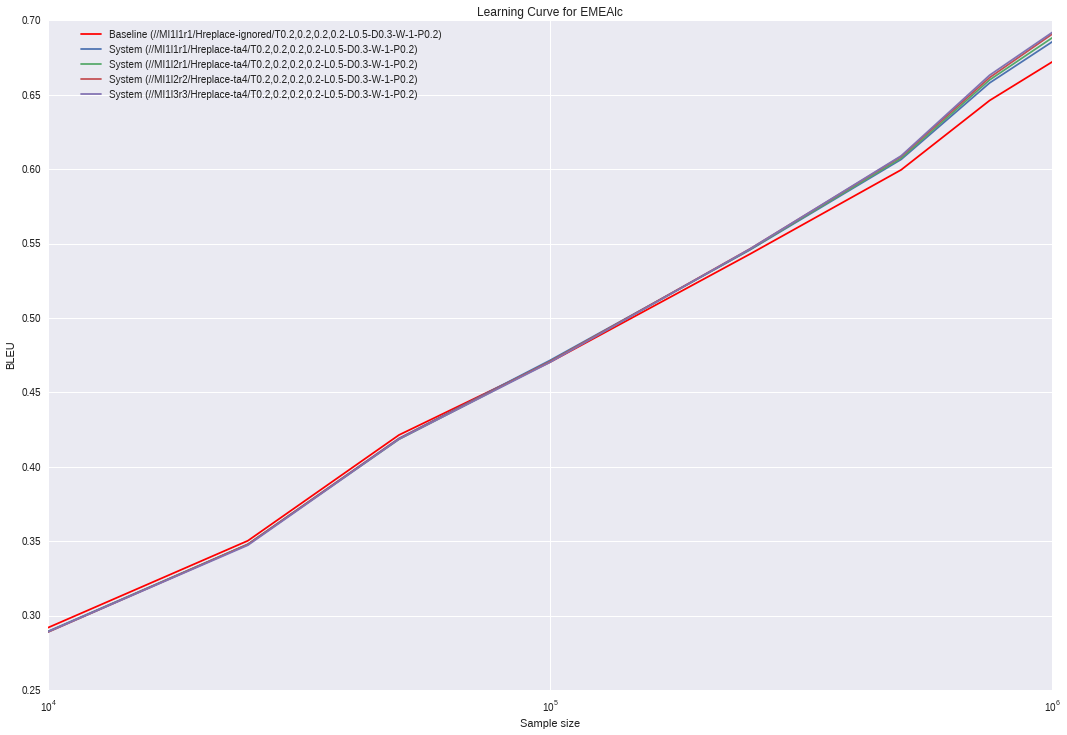
\includegraphics[width=120.00mm]{emealcbleu.png}
\caption{Learning curve on EMEA, English to Spanish, measuring BLEU score, logarithmic scale}
\label{fig:emealc}
\end{figure}


\begin{figure}
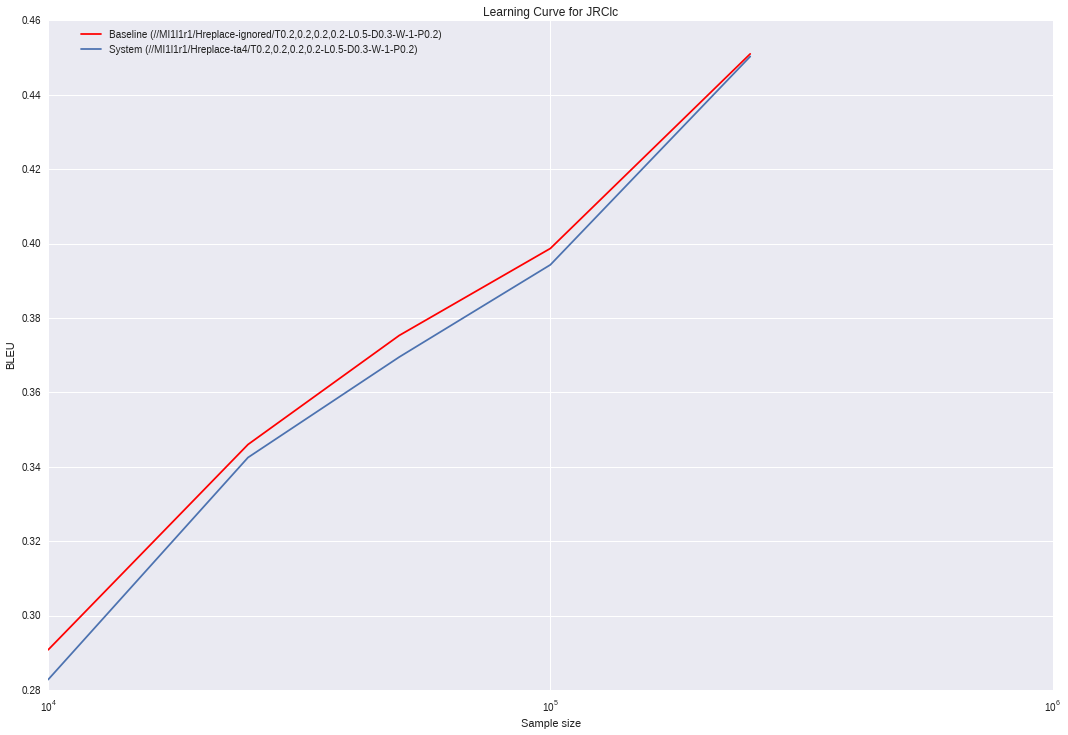
\includegraphics[width=120.00mm]{jrclcbleu.png}
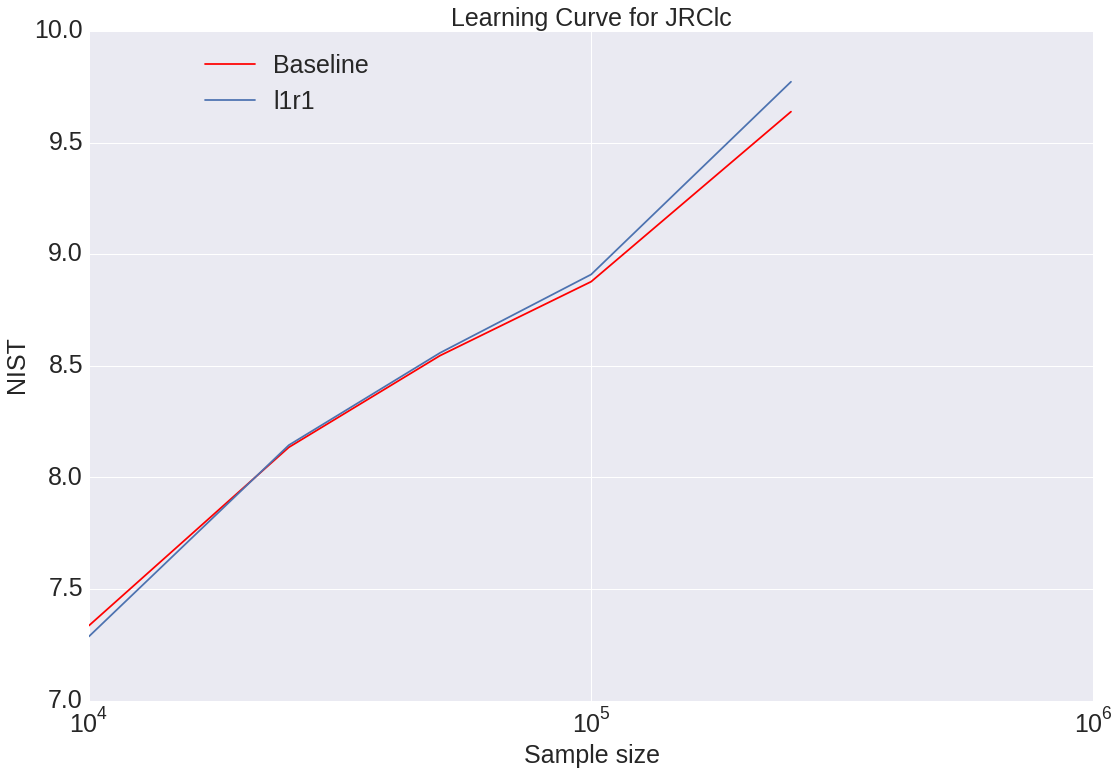
\includegraphics[width=120.00mm]{jrclcnist.png}
\caption{Learning curve on JRC Acquis, English to Spanish, measuring BLEU score (top) and NIST (bottom), logarithmic scale}
\label{fig:jrclc}
\end{figure}


In the EMEA learning curve in Table~\ref{fig:emealc}, we included an analysis
of different context sizes.  An enlargement of the context size seems to be
beneficial for this data set each step along the way, but these results have
already been shown not to generalise easily, nor is this trend likely to
continue if ever more context were to be added.

The positive results on the EMEA and JRC data needs to be contrasted to the
earlier negative results. Can we identify why these corpora, with these
language pairs, perform well?

We can observe that the nature of these two corpora consists of highly
formulaic language, medical language in the case of EMEA, and judicial language
in the case of JRC-Acquis.  This is implies the language is generally more
rigidly structured, predictable, and therefore easier to translate than corpora
from more diverse domains. The fact that the scores for these corpora are
higher than those for the corpora we've seen before illustrates this point.

As hypothesised earlier, it may be possible that a certain quality of
translation is needed before the source-side context information is able to
make an impact. The learning curve experiments suggest this, but it is at odds
with the positive results on the Chinese-English IWSLT 2006 data
(Table~\ref{tab:iwslt2006zhen}), which shows lower scores and is trained on a very
small training set. We dive further into this hypothesis with a series of
experiments on a Dutch-Frisian corpus. The high similarity between these two
Germanic languages of The Netherlands makes translation easier, and has been
shown to achieve high scores \citep{OERSETTER}. Table~\ref{tab:fa2} shows our
findings. Although high scores were obtained as expected, we were completely
unable to exceed the non-context-informed baseline. 

\begin{table}
\begin{tabular}{|l|ccccc|}
\hline
\textbf{System} & \textsc{BLEU}  & \textsc{METEOR}  & \textsc{NIST}  & \textsc{WER}  & \textsc{PER}  \\ 
\hline
\multicolumn{6}{|c|}{Fryske Akademy -- Frisian$\rightarrow$Dutch} \\
\hline 
Baseline (replace/M/opt) & \textbf{0.5572} & \textbf{0.7084} & \textbf{10.3162} & \textbf{29.86} & \textbf{24.73} \\ 
l1r1 (monolithic/replace/opt/tribl2) & 0.5544 & 0.7066 & 10.2967 & 30.08 & 24.91 \\ 
l1r1 (experts/replace/opt/ib1) & 0.5566 & 0.7077 & 10.3136 & 29.96 & 24.81 \\ 
\hline
\multicolumn{6}{|c|}{Fryske Akademy -- Dutch$\rightarrow$Frisian} \\
\hline
Baseline (replace/M/opt) & \textbf{0.5222} & \textbf{0.6911} & \textbf{9.9762} & \textbf{32.68} & \textbf{27.28} \\ 
l1r1 (monolithic/replace/opt/tribl2) & 0.5154 & 0.6857 & 9.9122 & 33.09 & 27.71 \\ 
l1r1 (experts/replace/opt/ib1) & 0.5164 & 0.6869 & 9.9258 & 33.0 & 27.59 \\ 
l2r1 (monolithic/replace/opt/tribl2) & 0.5145 & 0.6849 & 9.8992 & 33.16 & 27.78 \\ 
l2r1 (experts/replace/opt/ib1) & 0.5155 & 0.6864 & 9.9110 & 33.05 & 27.65 \\ 
l2r2 (monolithic/replace/opt/tribl2) & 0.5130 & 0.6841 & 9.8885 & 33.28 & 27.84 \\ 
l2r2 (experts/replace/opt/ib1) & 0.5157 & 0.6866 & 9.9159 & 33.05 & 27.61 \\ 
l3r3 (monolithic/replace/opt/tribl2) & 0.5114 & 0.6832 & 9.8656 & 33.41 & 27.97 \\ 
l3r3 (experts/replace/opt/ib1) & 0.5134 & 0.6852 & 9.8908 & 33.21 & 27.79 \\ 
\hline
\end{tabular}
\caption{Results on the Frisian-Dutch parallel corpus}
\label{tab:fa2}
\end{table}


We further address the issue of domain in a cross-domain experiment, to assess
whether introducing a differentiation between domains has a positive impact
when source-side context information is included. We did this for Dutch to
English, trained on 250,000 instances of the Europarl parallel corpus, and
tested on the IWSLT 2012 TED data. We find the context-informed
system\footnote{l1r1 (monolithic/replace/uni/tribl2)} scoring the
same\footnote{BLEU 0.2137, METEOR 0.4798, NIST 6.2172, WER 57.99, PER 46.01} as
the baseline, and thus not providing any added value. Unsurprisingly, scores
are considerably lower than when tested on the same domain (c.f
Table~\ref{tab:europarl250k}).

The below-baseline results for Dutch-English on two corpora (Europarl and IWSLT
2012 TED) may suggest that the efficacy of source-side context modelling
depends strongly on the language pair. A possible hypothesis here is that
source-side context modelling stands to gain most when translation from
morphologically simpler languages to morphologically richer languages, as the
source-side context information may help in determining the proper
morphological form. 

We test this hypothesis by conducting two experiments. All of the positive
results hitherto have been on language pairs in which the target language was
morphologically richer.  In the first experiment we therefore take such a
language pair, the English to Spanish language pair, and use it for a corpus
that has performed poorly: the 250,000 sentence subset of Europarl.  If the
results are better with English to Spanish than with Dutch to English then our
hypothesis would be strengthens our hypothesis. When we look at the results of
this experiment in Table~\ref{tab:europarl250k}, however, we immediately see
that this is not the case; all results are below baseline. A possible
explanation may be that more training data is needed, as suggested by the
earlier learning curves, but this too was an hypothesis we could not confirm on
another data set.

\begin{table}
\begin{tabular}{|l|ccccc|}
\textbf{System} & \textsc{BLEU}  & \textsc{METEOR}  & \textsc{NIST}  & \textsc{WER}  & \textsc{PER}  \\ 
\hline
\multicolumn{6}{c}{Europarl 250k - English $\rightarrow$ Spanish} \\
\hline 
Baseline (replace/M/opt) & \textbf{0.3424} & \textbf{0.5718} & 7.9896 & 53.64 & 39.2 \\ 
l1r1 (monolithic/replace/opt/tribl2) & 0.336 & 0.5666 & 7.9981 & 53.6 & 39.27 \\ 
l1r1 (experts/replace/opt/ib1) & 0.338 & 0.5677 & \textbf{8.0165} & \textbf{53.48} & \textbf{39.19} \\ 
l2r1 (monolithic/replace/opt/tribl2) & 0.3344 & 0.5651 & 7.993 & 53.63 & 39.3 \\ 
l2r1 (experts/replace/opt/ib1) & 0.3357 & 0.5664 & 8.0086 & 53.51 & 39.23 \\ 
l2r2 (monolithic/replace/opt/tribl2) & 0.3325 & 0.5639 & 7.9843 & 53.6 & 39.36 \\ 
l2r2 (experts/replace/opt/ib1) & 0.3345 & 0.5649 & 8.0 & 53.55 & 39.32 \\ 
l3r3 (monolithic/replace/opt/tribl2) & 0.329 & 0.5611 & 7.9518 & 53.74 & 39.61 \\ 
l3r3 (experts/replace/opt/ib1) & 0.3298 & 0.562 & 7.9593 & 53.79 & 39.57 \\ 
\hline
\end{tabular}
\caption{Negative results on Europarl 250k - English to Spanish}
\label{tab:europarl250k}
\end{table}

The second attempt to test this hypothesis focusses on English to Russian, a
very morphologically rich language with three genders and six cases. Under our
hypothesis, we would expect positive results here.  Table~\ref{tab:yandex1M}
shows the results of this experiment.

\todo{TODO: wait for english-russian, process results and draw conclusion}



\subsection{Results: classifier type and classifier parameter optimisation}
\label{sec:typeopt}

We have introduced two types of classifier, integrated in an Statistical
Machine Translation framework by means of the ``bypass'' method described in
Section~\ref{sec:smtintegration}. The monolithic classifier, modelling all phrase-pairs
in a single classifier, is used also by \cite{Stroppa+07} and
\cite{Rejwanul+11}, whereas the classifiers experts, one classifier per
source-phrase, is a new addition that more closely resembles how such
classifiers are employed in Word Sense Disambiguation.

Classifier experts were built using the IB1 algorithm, whereas we choose for
TRIBL2 for the monolithic classifier. This was done because the monolithic
classifier is a lot bigger by definition, and therefore the high performance of
the algorithm IGTree becomes imperative, a pure IB1 approach would be too slow
and TRIBL2 seeks to combine the best of both worlds.

Table~\ref{tab:expertcount} lists the number of classifier experts that were
built for some of the data sets. The actual number of source phrases is always
much higher, as classifiers are only built when there is ambiguity regarding
the translation. To see how these classifiers are typically distributed, based
on the number of instances and classes, we zoom in on the IWSLT 2012 data for
Dutch to English, and plot a histogram in Figure~\ref{fig:histogram}. As is
ubiquitous in natural language processing, a zipf curve can be discerned from
this figure, with the vast majority of classifier experts being very small and
having few translations options, i.e classes, and an immediate sharp drop in
frequency as the number of instances or classes increases.

\begin{table}
\begin{tabular}{|lll|l|}
\hline
\textbf{Corpus} & \textbf{Sentence pairs} & \textbf{Languages} & \textbf{Classifier Experts} \\
\hline
Europarl & 250,000 & English-Spanish & 828,326 \\
JRC & 250,000 & English-Spanish & 635,547 \\
IWSLT 2012 TED & 127,806 & Dutch-English & 193,811 \\
IWSLT 2006 & 40,274 & Chinese-English & 22,212 \\
Fryske Akademy & 137,937 & Dutch-Frisian & 276,819 \\
Fryske Akademy & 137,937 & Frisian-Dutch & 213,573 \\
\hline
\end{tabular}
\caption{Number of classifier experts generated per data set}
\label{tab:expertcount}
\end{table}


\begin{figure}
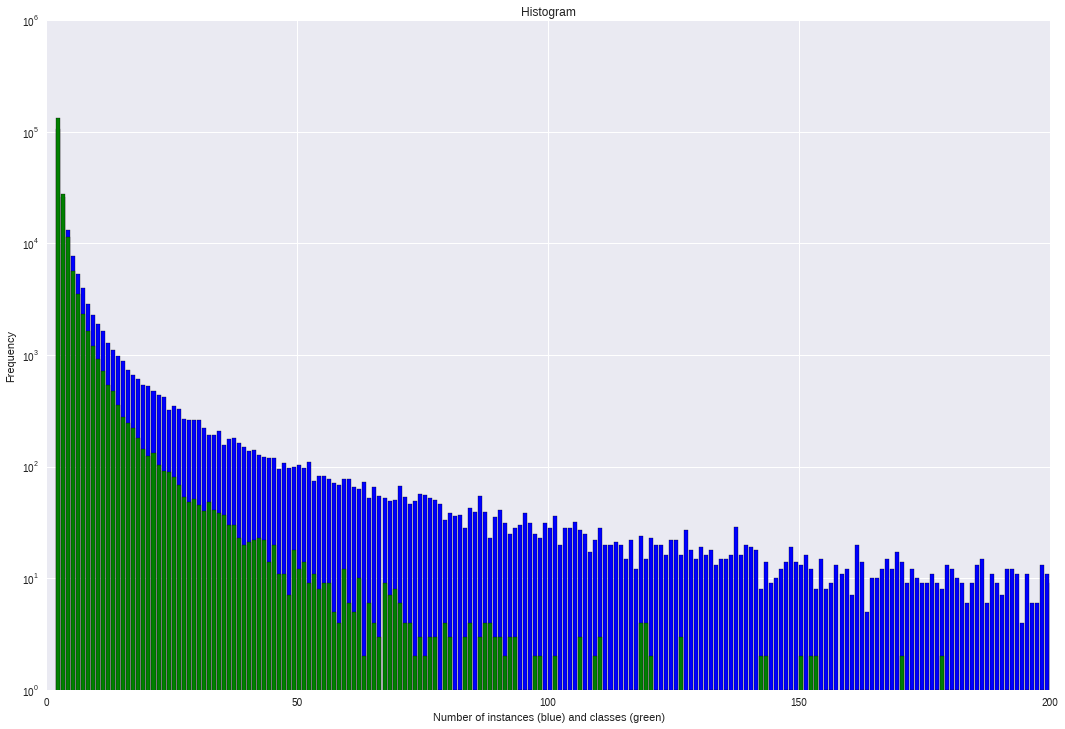
\includegraphics[width=80.00mm]{classifierhistogram.png}
\caption{Histogram showing the distribution of the number of instances (blue) and number of classes (green) in the classifier experts for IWSLT 2012 TED, Dutch to English (logarithmic)}
\label{fig:histogram}
\end{figure}

Most of the tables in Section~\ref{sec:results1} list results for both classifier
types.  We find the classifier experts outperforming the monolithic classifier
for Chinese-English (Table~\ref{tab:iwslt2006zhen} (for all context sizes except
\texttt{l3r3}), for  IWSTL 2012 TED Dutch-English (Table~\ref{tab:iwslt2012},
mostly below baseline), Europarl250k Dutch-English
(Table~\ref{tab:europarl250k}, mostly below baseline), and Frisian-Dutch
(Table~\ref{tab:fa2}, all below baseline)).

These results suggest that the classifier experts perform better than the
monolithic classifier. When looking at the two 250,000 instance samples of
JRC-Acquis (Table~\ref{tab:jrc250k}), we see a conflicting image. One sample
confirms our hypothesis that the classifier experts are better, whereas in the
other the monolithic classifier has the upper-hand. Moreover, when we look at
the EMEA data (Table~\ref{tab:emea}), where we had the most significant gains
above baseline, we find the monolithic system strongest. 

Despite the results not being unanimous, the case for the classifier experts is
strong and can be motivated by the fact that feature weights are computed on a per-
source-phrase basis, rather than on the aggregation of all. It can be considered as a
kind of optimisation step. The disadvantage is that such systems may therefore
be more prone to overfitting on one hand, which might well be the case in the
EMEA experiment, as well as sparsity problems for smaller classifier experts on
the other hand.

\todo{TODO: parameter optimisation experiment (still to run and process)}


\subsection{Results: Weighting methods and score analysis}
\label{sec:weighting}

Two weighting methods have been implemented, the \emph{append} method, adding
$p(t|s,C)$ as an extra score to the score vector, and the \emph{replace}
method, which replaces the existing $p(t|s)$ score with $p(t|s,C)$. Most
experiments have been conducted with the \emph{replace} method, as it is the
simplest one. For EMEA (Table~\ref{tab:emea}) and JRC-Acquis
(Table~\ref{tab:jrc250k}), the \emph{append} method was tested as well.

Comparing the two weighting methods, however, is far from trivial. When a
discrepancy is found between a run with the replace method (4 scores) and the
run with the append method (5 scores), we can not simply ascribe such a
difference to the extra score, but must into account that the very act of
adding a score shifts the weights for the score vector, even if uniformly
distributed. Any shift may likely affect the outcome. This
motivation is also the reason we included a separate baseline for the append
method in the tables in which we reported it. Moreover, it explains why we can
not just apply the results of the parameter optimisation of the replace method
to the append method.

Tables~\ref{tab:emea} (EMEA) and \ref{tab:jrc250k} (JRC) have been run without
parameter optimisation. Even without context information, the baselines for the
append method score better than those for the replace method. Effectively, the
append method's baseline is simply a version with a double feature and
functionally equivalent to just assigning double weight to the feature.

A comparison is complicated by the fact that the $p(t|s,C)$ score is often simply
equal to the $p(t|s)$ score, by definition so for any source phrases for which no
classifier was needed, due to not being ambiguous in translation or context. 

We can therefore not draw any satisfactory conclusions on the merit of the
\emph{append} method versus the \emph{replace} method, given the experiments we
conducted. We can, however, use the two different scoring methods to provide
insight into the classifier results. How often does the classifier assign a
$P(t|s,C)$ that significantly differs from $P(t|s)$? And how often are they
completely identical?

Such an analysis has been conducted on the test data of the JRC-Acquis
corpus,from English to Spanish. This is shown in
Figure~\ref{fig:scoredifference}. 

For each occurrence of each source phrase in the test-data, we gathered all
possible translations and computed $\frac{P(t|s,C)}{P(t|s)}$. This ratio
expresses the difference between the context-informed translation probability
and the non-context informed one.

A value of one indicates there is no difference whatsoever, this includes all
source phrases where either translation or context are unambiguous. A spike can
be observed at this point, this spike covers $9\%$ of phrase-pairs. The right
hand side of the graph ($>1$), is of most interest, it covers the phrase-pairs
for which the classifier increased the probability, we compute that $75\%$ of
the phrase-pairs is in this region, which is reflected by the increased
noise in the graph. 

%A downward trend can be observed in the graph, downward adjustments are more
%prevalent as it it is a logical consequence of increasing probability to one
%translation over the others in a distribution.

\begin{figure}
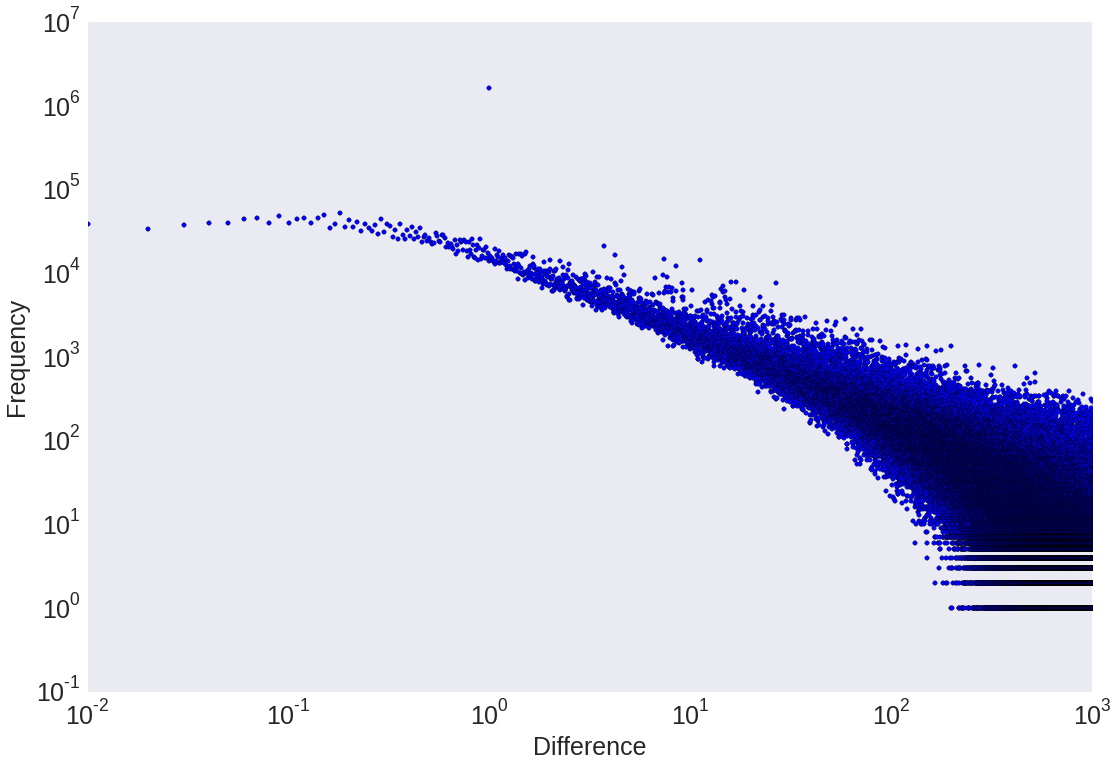
\includegraphics[width=80.00mm]{scoredifference.png}
\caption{Histogram in logarithmic scale showing the ratio $\frac{P(t|s,C)}{P(t|s)}$ for JRC250k English to Spanish test set, illustrating the difference between the classifier score and the original SMT score.}
\label{fig:scoredifference}
\end{figure}


\todo{TODO: continue/rethink analysis of difference between  $P(t|s)$ and $P(t|s,C)$ scores}

\subsection{Results: Qualitative Analysis}

In this section we will take a look at the translations themselves and see if
we can discern patterns that can tell us what the effect of source-side context
information is and when it pays off.

We zoom in on the corpus that performed best, the EMEA corpus -- English to
Spanish, one million sentence pairs. We compare the context-informed
\texttt{l1r1} system with the non-context informed baseline to assess the
impact of the context information. Out of $5000$ sentences in the test set,
$3863$ ($77\%$) are translated identically. This high number again shows that
it is difficult to make a difference. Nevertheless, $22\%$ differs and results
in a net gain in translation performance, as seen in Table~\ref{tab:EMEA}.

The next few examples will show some comparisons in which the context-informed
improves over the baseline. 

Example~\ref{ex:QAsynonym} shows three examples of the selection of a better
translation given the context, matching with the reference translation, even
though the baseline translation could be considered correct as well. This is
the most common type of difference. Example~\ref{ex:QAdrop} shows the dropping
of a word.


\begin{exmp}
\footnotesize
\label{ex:QAsynonym}
\textbf{Baseline:} El cambio continuo del lugar de inyección dentro de \underline{un área} determinada puede ayudar a \\
\textbf{l1r1:} El cambio continuo del lugar de inyección dentro de \underline{una región} determinada puede ayudar a \\
\textbf{Reference:} La contínua rotación de los puntos de inyección dentro de \underline{una región} determinada puede ayudar a reducir o prevenir estas reacciones \\
\noindent\makebox[\linewidth]{\rule{\linewidth}{0.4pt}}
\textbf{Baseline:} Baraclude reduce la cantidad de virus en su \underline{cuerpo} y mejora el estado del hígado . \\
\textbf{l1r1:} Baraclude reduce la cantidad de virus en su \underline{organismo} y mejora el estado del hígado  \\
\textbf{Reference:} Baraclude reduce la cantidad de virus en su \underline{organismo} y mejora el estado del hígado .
\\ 
\noindent\makebox[\linewidth]{\rule{\linewidth}{0.4pt}}
\textbf{Baseline:} Como consecuencia , el fenilbutirato de sodio , reduce \underline{los niveles plasmáticos} de amonio y glutamina en pacientes con trastornos del ciclo de la urea . \\
\textbf{l1r1:} Como consecuencia , el fenilbutirato de sodio reduce \underline{las concentraciones plasmáticas elevadas} de amonio y glutamina en pacientes con trastornos del ciclo de la urea .  \\
\textbf{Reference:} Como consecuencia , el fenilbutirato de sodio reduce \underline{las concentraciones plasmáticas elevadas} de amoníaco y glutamina en pacientes con trastornos del ciclo de la urea .
\end{exmp}

\begin{exmp}
\footnotesize
\label{ex:QAdrop}
\textbf{Baseline:} \underline{Los estudios} en animales , no pueden excluir el desarrollo potencial de toxicidad ( ver sección 5.3 ) . \\
\textbf{l1r1:} \underline{Estudios} en animales , no pueden excluir el desarrollo potencial de toxicidad ( ver sección 5.3 ) . \\
\textbf{Reference:} \underline{Estudios} en animales , no pueden excluir el desarrollo potencial de toxicidad ( ver sección 5.3 ) .
\end{exmp}

\begin{exmp}
\footnotesize
\label{ex:QAgrammar}
\textbf{Baseline:} Las reacciones adversas \underline{consideradas relacionadas} con el uso de Agenerase son síntomas gastrointestinales , erupción y parestesia oral / peri-oral . \\
\textbf{l1r1:}  Las reacciones adversas \underline{que se consideran relacionadas} con el uso de Agenerase son síntomas gastrointestinales , erupción y parestesia oral / \\
\textbf{Reference:} Las reacciones adversas \underline{que se consideran relacionadas} con el uso de Agenerase son síntomas gastrointestinales , erupción y parestesia oral / perioral . \\ \\
\end{exmp}

In addition to the positive examples, there are also neutral and negative examples. In example~\ref{ex:QAneutral}, all translations can be considered correct and conveying the same message with different nuances, as a difference construction is chosen. Example~\ref{ex:QAnegative} shows the inverse situation of example~\ref{ex:QAsynonym}, a different synonym was chosen but it does not match with the reference translation. This too is a common pattern in the data. This raises the question whether the impact of context-information would not be lower if the test set would have contained multiple reference translations. Such data unfortunately is hard to come by and was not available in this study.

\begin{exmp}
\footnotesize
\label{ex:QAneutral}
\textbf{Baseline:} Asegúrese de que el polvo \underline{esté completamente disuelto} . \\
\textbf{l1r1:} Asegúrese de que el polvo \underline{se disuelva completamente} .  \\
\textbf{Reference:} Asegúrese de que el polvo \underline{se ha disuelto completamente} .
\end{exmp}

\begin{exmp}
\footnotesize
\label{ex:QAnegative}
\textbf{Baseline:} Los pacientes \underline{se asignaron aleatoriamente} a recibir 500 $\mu$ g de Aranesp una vez cada tres semanas o 2,25 $\mu$ g / kg una vez a la semana . \\
\textbf{l1r1:} Los pacientes \underline{fueron aleatorizados} a recibir 500 $\mu$ g de Aranesp una vez cada tres semanas o 2,25 $\mu$ g / kg una vez a la semana . \\
\textbf{Reference:} Los pacientes \underline{se asignaron aleatoriamente} a recibir 500 $\mu$ g de Aranesp una vez cada tres semanas o 2,25 $\mu$ g / kg una vez a la semana .
\end{exmp}


\section{Conclusion \& Discussion} 

We have conducted numerous experiments to assess whether source-side context
information, without the use of any explicit linguistic features that require
supervised parsers or taggers, can improve translation quality. Memory-based
classifiers were used, and integrated in an SMT framework. The
results of the experiments were mixed and there was a high degree of
variability between different corpora and language pairs. Positive results were
attained on EMEA and JRC-Acquis. 

We replicated part of the work of \cite{Stroppa+07} and \cite{Rejwanul+11}, and
found that results are fairly marginal. Inclusion of surface-form
source-side context information is clearly not the most obvious road for the
improvement of MT quality. It is likely that improvement can be more easily
achieved through simple improvement of the target-side language model.

In this discussion, we would like to focus on why the results of our study are
so marginal compared to baseline.  There is a theoretical foundation for this
if we look at the interplay between the SMT decoder and the classifiers. For a
source phrase $s$ with context $C$ and mapping to translation $t$ to be a
strong fragment in the classifier, it has to have been observed multiple times
in the training data. If this is so, then there is often a source fragment $s'$
in the phrase-translation table that is the conjunction of $s$ and $C$, and
which maps to a $t'$ of which $t$ is a substring. It is thus likely that the
context information we try to explicitly model, is often already implicitly
available to the decoder. This is provided that the classifier and
phrase-translation table are trained on the same parallel corpus, as we
consistently did.



\todo{TODO: finish}


\bibliographystyle{spbasic}
\bibliography{sourcecontextinsmt}




\end{document}
